% CVPR 2024 Paper Template; see https://github.com/cvpr-org/author-kit

\documentclass[10pt,twocolumn,letterpaper]{article}

%%%%%%%%% PAPER TYPE  - PLEASE UPDATE FOR FINAL VERSION
% \usepackage{cvpr}              % To produce the CAMERA-READY version
% \usepackage[review]{cvpr}      % To produce the REVIEW version
\usepackage[pagenumbers]{cvpr} % To force page numbers, e.g. for an arXiv version
\usepackage{lmodern,bm}
% Import additional packages in the preamble file, before hyperref
%
% --- inline annotations
%
\usepackage[dvipsnames]{xcolor}
\newcommand{\red}[1]{{\color{red}#1}}
\newcommand{\todo}[1]{{\color{red}#1}}
\newcommand{\TODO}[1]{\textbf{\color{red}[TODO: #1]}}
% --- disable by uncommenting  
% \renewcommand{\TODO}[1]{}
% \renewcommand{\todo}[1]{#1}



% It is strongly recommended to use hyperref, especially for the review version.
% hyperref with option pagebackref eases the reviewers' job.
% Please disable hyperref *only* if you encounter grave issues, 
% e.g. with the file validation for the camera-ready version.
%
% If you comment hyperref and then uncomment it, you should delete *.aux before re-running LaTeX.
% (Or just hit 'q' on the first LaTeX run, let it finish, and you should be clear).
\definecolor{cvprblue}{rgb}{0.21,0.49,0.74}
\usepackage[pagebackref,breaklinks,colorlinks,citecolor=cvprblue]{hyperref}

%%%%%%%%% PAPER ID  - PLEASE UPDATE
\def\paperID{*****} % *** Enter the Paper ID here
\def\confName{CVPR}
\def\confYear{2025}

%%%%%%%%% TITLE - PLEASE UPDATE
\title{Improving Cell Instance Segmentation with Test-Time Adaptation}

%%%%%%%%% AUTHORS - PLEASE UPDATE
\author{Quinn Jones \qquad Ram Zaveri \\
West Virginia University\\
% Institution1 address\\
{\tt\small \{qjones1, rz0012\}@mix.wvu.edu}
% For a paper whose authors are all at the same institution,
% omit the following lines up until the closing ``}''.
% Additional authors and addresses can be added with ``\and'',
% just like the second author.
% To save space, use either the email address or home page, not both
% \and
% Ram Zaveri\\
% Institution2\\
% First line of institution2 address\\
% {\tt\small secondauthor@i2.org}
}

\begin{document}
\maketitle
\begin{abstract}

\end{abstract}    
\section{Introduction}
\label{sec:intro}

Please follow the steps outlined below when submitting your manuscript to the IEEE Computer Society Press.
This style guide now has several important modifications (for example, you are no longer warned against the use of sticky tape to attach your artwork to the paper), so all authors should read this new version.

%-------------------------------------------------------------------------
\subsection{Language}

All manuscripts must be in English.

\subsection{Dual submission}

Please refer to the author guidelines on the \confName\ \confYear\ web page for a
discussion of the policy on dual submissions.

\subsection{Paper length}
Papers, excluding the references section, must be no longer than eight pages in length.
The references section will not be included in the page count, and there is no limit on the length of the references section.
For example, a paper of eight pages with two pages of references would have a total length of 10 pages.
{\bf There will be no extra page charges for \confName\ \confYear.}

Overlength papers will simply not be reviewed.
This includes papers where the margins and formatting are deemed to have been significantly altered from those laid down by this style guide.
Note that this \LaTeX\ guide already sets figure captions and references in a smaller font.
The reason such papers will not be reviewed is that there is no provision for supervised revisions of manuscripts.
The reviewing process cannot determine the suitability of the paper for presentation in eight pages if it is reviewed in eleven.

%-------------------------------------------------------------------------
\subsection{The ruler}
The \LaTeX\ style defines a printed ruler which should be present in the version submitted for review.
The ruler is provided in order that reviewers may comment on particular lines in the paper without circumlocution.
If you are preparing a document using a non-\LaTeX\ document preparation system, please arrange for an equivalent ruler to appear on the final output pages.
The presence or absence of the ruler should not change the appearance of any other content on the page.
The camera-ready copy should not contain a ruler.
(\LaTeX\ users may use options of \texttt{cvpr.sty} to switch between different versions.)

Reviewers:
note that the ruler measurements do not align well with lines in the paper --- this turns out to be very difficult to do well when the paper contains many figures and equations, and, when done, looks ugly.
Just use fractional references (\eg, this line is $087.5$), although in most cases one would expect that the approximate location will be adequate.


\subsection{Paper ID}
Make sure that the Paper ID from the submission system is visible in the version submitted for review (replacing the ``*****'' you see in this document).
If you are using the \LaTeX\ template, \textbf{make sure to update paper ID in the appropriate place in the tex file}.


\subsection{Mathematics}

Please number all of your sections and displayed equations as in these examples:
\begin{equation}
  E = m\cdot c^2
  \label{eq:important}
\end{equation}
and
\begin{equation}
  v = a\cdot t.
  \label{eq:also-important}
\end{equation}
It is important for readers to be able to refer to any particular equation.
Just because you did not refer to it in the text does not mean some future reader might not need to refer to it.
It is cumbersome to have to use circumlocutions like ``the equation second from the top of page 3 column 1''.
(Note that the ruler will not be present in the final copy, so is not an alternative to equation numbers).
All authors will benefit from reading Mermin's description of how to write mathematics:
\url{http://www.pamitc.org/documents/mermin.pdf}.

\subsection{Blind review}

Many authors misunderstand the concept of anonymizing for blind review.
Blind review does not mean that one must remove citations to one's own work---in fact it is often impossible to review a paper unless the previous citations are known and available.

Blind review means that you do not use the words ``my'' or ``our'' when citing previous work.
That is all.
(But see below for tech reports.)

Saying ``this builds on the work of Lucy Smith [1]'' does not say that you are Lucy Smith;
it says that you are building on her work.
If you are Smith and Jones, do not say ``as we show in [7]'', say ``as Smith and Jones show in [7]'' and at the end of the paper, include reference 7 as you would any other cited work.

An example of a bad paper just asking to be rejected:
\begin{quote}
\begin{center}
    An analysis of the frobnicatable foo filter.
\end{center}

   In this paper we present a performance analysis of our previous paper [1], and show it to be inferior to all previously known methods.
   Why the previous paper was accepted without this analysis is beyond me.

   [1] Removed for blind review
\end{quote}


An example of an acceptable paper:
\begin{quote}
\begin{center}
     An analysis of the frobnicatable foo filter.
\end{center}

   In this paper we present a performance analysis of the  paper of Smith \etal [1], and show it to be inferior to all previously known methods.
   Why the previous paper was accepted without this analysis is beyond me.

   [1] Smith, L and Jones, C. ``The frobnicatable foo filter, a fundamental contribution to human knowledge''. Nature 381(12), 1-213.
\end{quote}

If you are making a submission to another conference at the same time, which covers similar or overlapping material, you may need to refer to that submission in order to explain the differences, just as you would if you had previously published related work.
In such cases, include the anonymized parallel submission~\cite{Authors14} as supplemental material and cite it as
\begin{quote}
[1] Authors. ``The frobnicatable foo filter'', F\&G 2014 Submission ID 324, Supplied as supplemental material {\tt fg324.pdf}.
\end{quote}

Finally, you may feel you need to tell the reader that more details can be found elsewhere, and refer them to a technical report.
For conference submissions, the paper must stand on its own, and not {\em require} the reviewer to go to a tech report for further details.
Thus, you may say in the body of the paper ``further details may be found in~\cite{Authors14b}''.
Then submit the tech report as supplemental material.
Again, you may not assume the reviewers will read this material.

Sometimes your paper is about a problem which you tested using a tool that is widely known to be restricted to a single institution.
For example, let's say it's 1969, you have solved a key problem on the Apollo lander, and you believe that the 1970 audience would like to hear about your
solution.
The work is a development of your celebrated 1968 paper entitled ``Zero-g frobnication: How being the only people in the world with access to the Apollo lander source code makes us a wow at parties'', by Zeus \etal.

You can handle this paper like any other.
Do not write ``We show how to improve our previous work [Anonymous, 1968].
This time we tested the algorithm on a lunar lander [name of lander removed for blind review]''.
That would be silly, and would immediately identify the authors.
Instead write the following:
\begin{quotation}
\noindent
   We describe a system for zero-g frobnication.
   This system is new because it handles the following cases:
   A, B.  Previous systems [Zeus et al. 1968] did not  handle case B properly.
   Ours handles it by including a foo term in the bar integral.

   ...

   The proposed system was integrated with the Apollo lunar lander, and went all the way to the moon, don't you know.
   It displayed the following behaviours, which show how well we solved cases A and B: ...
\end{quotation}
As you can see, the above text follows standard scientific convention, reads better than the first version, and does not explicitly name you as the authors.
A reviewer might think it likely that the new paper was written by Zeus \etal, but cannot make any decision based on that guess.
He or she would have to be sure that no other authors could have been contracted to solve problem B.
\medskip

\noindent
FAQ\medskip\\
{\bf Q:} Are acknowledgements OK?\\
{\bf A:} No.  Leave them for the final copy.\medskip\\
{\bf Q:} How do I cite my results reported in open challenges?
{\bf A:} To conform with the double-blind review policy, you can report results of other challenge participants together with your results in your paper.
For your results, however, you should not identify yourself and should not mention your participation in the challenge.
Instead present your results referring to the method proposed in your paper and draw conclusions based on the experimental comparison to other results.\medskip\\

\begin{figure}[t]
  \centering
  \fbox{\rule{0pt}{2in} \rule{0.9\linewidth}{0pt}}
   %\includegraphics[width=0.8\linewidth]{egfigure.eps}

   \caption{Example of caption.
   It is set in Roman so that mathematics (always set in Roman: $B \sin A = A \sin B$) may be included without an ugly clash.}
   \label{fig:onecol}
\end{figure}

\subsection{Miscellaneous}

\noindent
Compare the following:\\
\begin{tabular}{ll}
 \verb'$conf_a$' &  $conf_a$ \\
 \verb'$\mathit{conf}_a$' & $\mathit{conf}_a$
\end{tabular}\\
See The \TeX book, p165.

The space after \eg, meaning ``for example'', should not be a sentence-ending space.
So \eg is correct, {\em e.g.} is not.
The provided \verb'\eg' macro takes care of this.

When citing a multi-author paper, you may save space by using ``et alia'', shortened to ``\etal'' (not ``{\em et.\ al.}'' as ``{\em et}'' is a complete word).
If you use the \verb'\etal' macro provided, then you need not worry about double periods when used at the end of a sentence as in Alpher \etal.
However, use it only when there are three or more authors.
Thus, the following is correct:
   ``Frobnication has been trendy lately.
   It was introduced by Alpher~\cite{Alpher02}, and subsequently developed by
   Alpher and Fotheringham-Smythe~\cite{Alpher03}, and Alpher \etal~\cite{Alpher04}.''

This is incorrect: ``... subsequently developed by Alpher \etal~\cite{Alpher03} ...'' because reference~\cite{Alpher03} has just two authors.

\begin{figure*}
  \centering
  \begin{subfigure}{0.68\linewidth}
    \fbox{\rule{0pt}{2in} \rule{.9\linewidth}{0pt}}
    \caption{An example of a subfigure.}
    \label{fig:short-a}
  \end{subfigure}
  \hfill
  \begin{subfigure}{0.28\linewidth}
    \fbox{\rule{0pt}{2in} \rule{.9\linewidth}{0pt}}
    \caption{Another example of a subfigure.}
    \label{fig:short-b}
  \end{subfigure}
  \caption{Example of a short caption, which should be centered.}
  \label{fig:short}
\end{figure*}

\section{Related Works}
\label{sec:RW}
To discuss the related works we will discuss the challenges of Cell Segmentation and Test-Time Adaptation (TTA).

\subsection{Cell Segmentation}

Cell segmentation is the process of taking images from a microscope and automatically labelling each pixel of the image as belonging to a cell or not (in other words a background pixel).  For the purposes of tracking generally we take this a step further and perform instance segmentation~\cite{Yang_2019_ICCV}.  Instance segmentation adds the extra goal of keeping a separate label for each of the objects of interest.  \\ 

A recent leader in that field is~\cite{bragantini2024ucmtracking}.  In~\cite{bragantini2024ucmtracking}, the authors designed their algorithm specifically for fluorescent imaging techniques, but their hierarchical technique facilitates holding multiple hypotheses for the tracking which means they are much more prepared for the cell division and death mentioned in \ref{sec:intro}.  The tools to work at scale aren't available as generalized algorithm for locating  single cells in images don't yet exist, as backed up by~\cite{greenwald2022whole}.


\subsection{Test-Time Adaptation}
\label{sec:TTARW}

TTA is a method that attempts to solve the issue of drift in the data distribution between the training and testing data. This serves the purpose of making a model that is generalizable which is especially valuable for medical imaging due to its variability. 
\\

Our approach to test-time adaptation follows in the footsteps of~\cite{Li2018-el}, which introduced batch normalization in test-time adaptation. In~\cite{Li2018-el}, they present \textit{AdaBN}, where they use the property of eliminating covariate shift that BN was originally built for by collecting the batch normalizing statistics of the whole of the target domain before re-classifying with the optimized settings.  This becomes an even more powerful tool when combined with more in-depth criteria for the BN settings.  Such as ~\cite{wang2020tent} which we mirror where they use the Shannon entropy of the model predictions to learn an affine transformation that shifts the output following the normalization.  We improve on it further by adding a simultaneous contrastive flow loss to affect the speed of convergence.\\

In ~\cite{chen2024cmtt,Moshkov2020-uy} recently they apply TTA to cell image tracking/segmentation in different ways.  In~\cite{chen2024cmtt} a central-metric contrastive loss is used to break the image into patches and adapt them separately and simultaneously to the whole image adaptation.  By breaking the problem into two, but aggregating the information back into one pre-segmentation they improve their false-negative rates as the hardest, most off-distribution samples are overlooked.   In~\cite{Moshkov2020-uy} the adaptation happens at the input with a system that feeds the input datum augmented by rotations, translations, and/or flipped.  The original and all of the augmented samples are processed by the network and then the outputs are dis-augmented, for instance if the input was flipped along the x-y axis the output would be flipped again to undo the transformation.  This way biases in the orientation of features in the training data can be averaged out.  





\section{Problem Definition}
\begin{figure}
    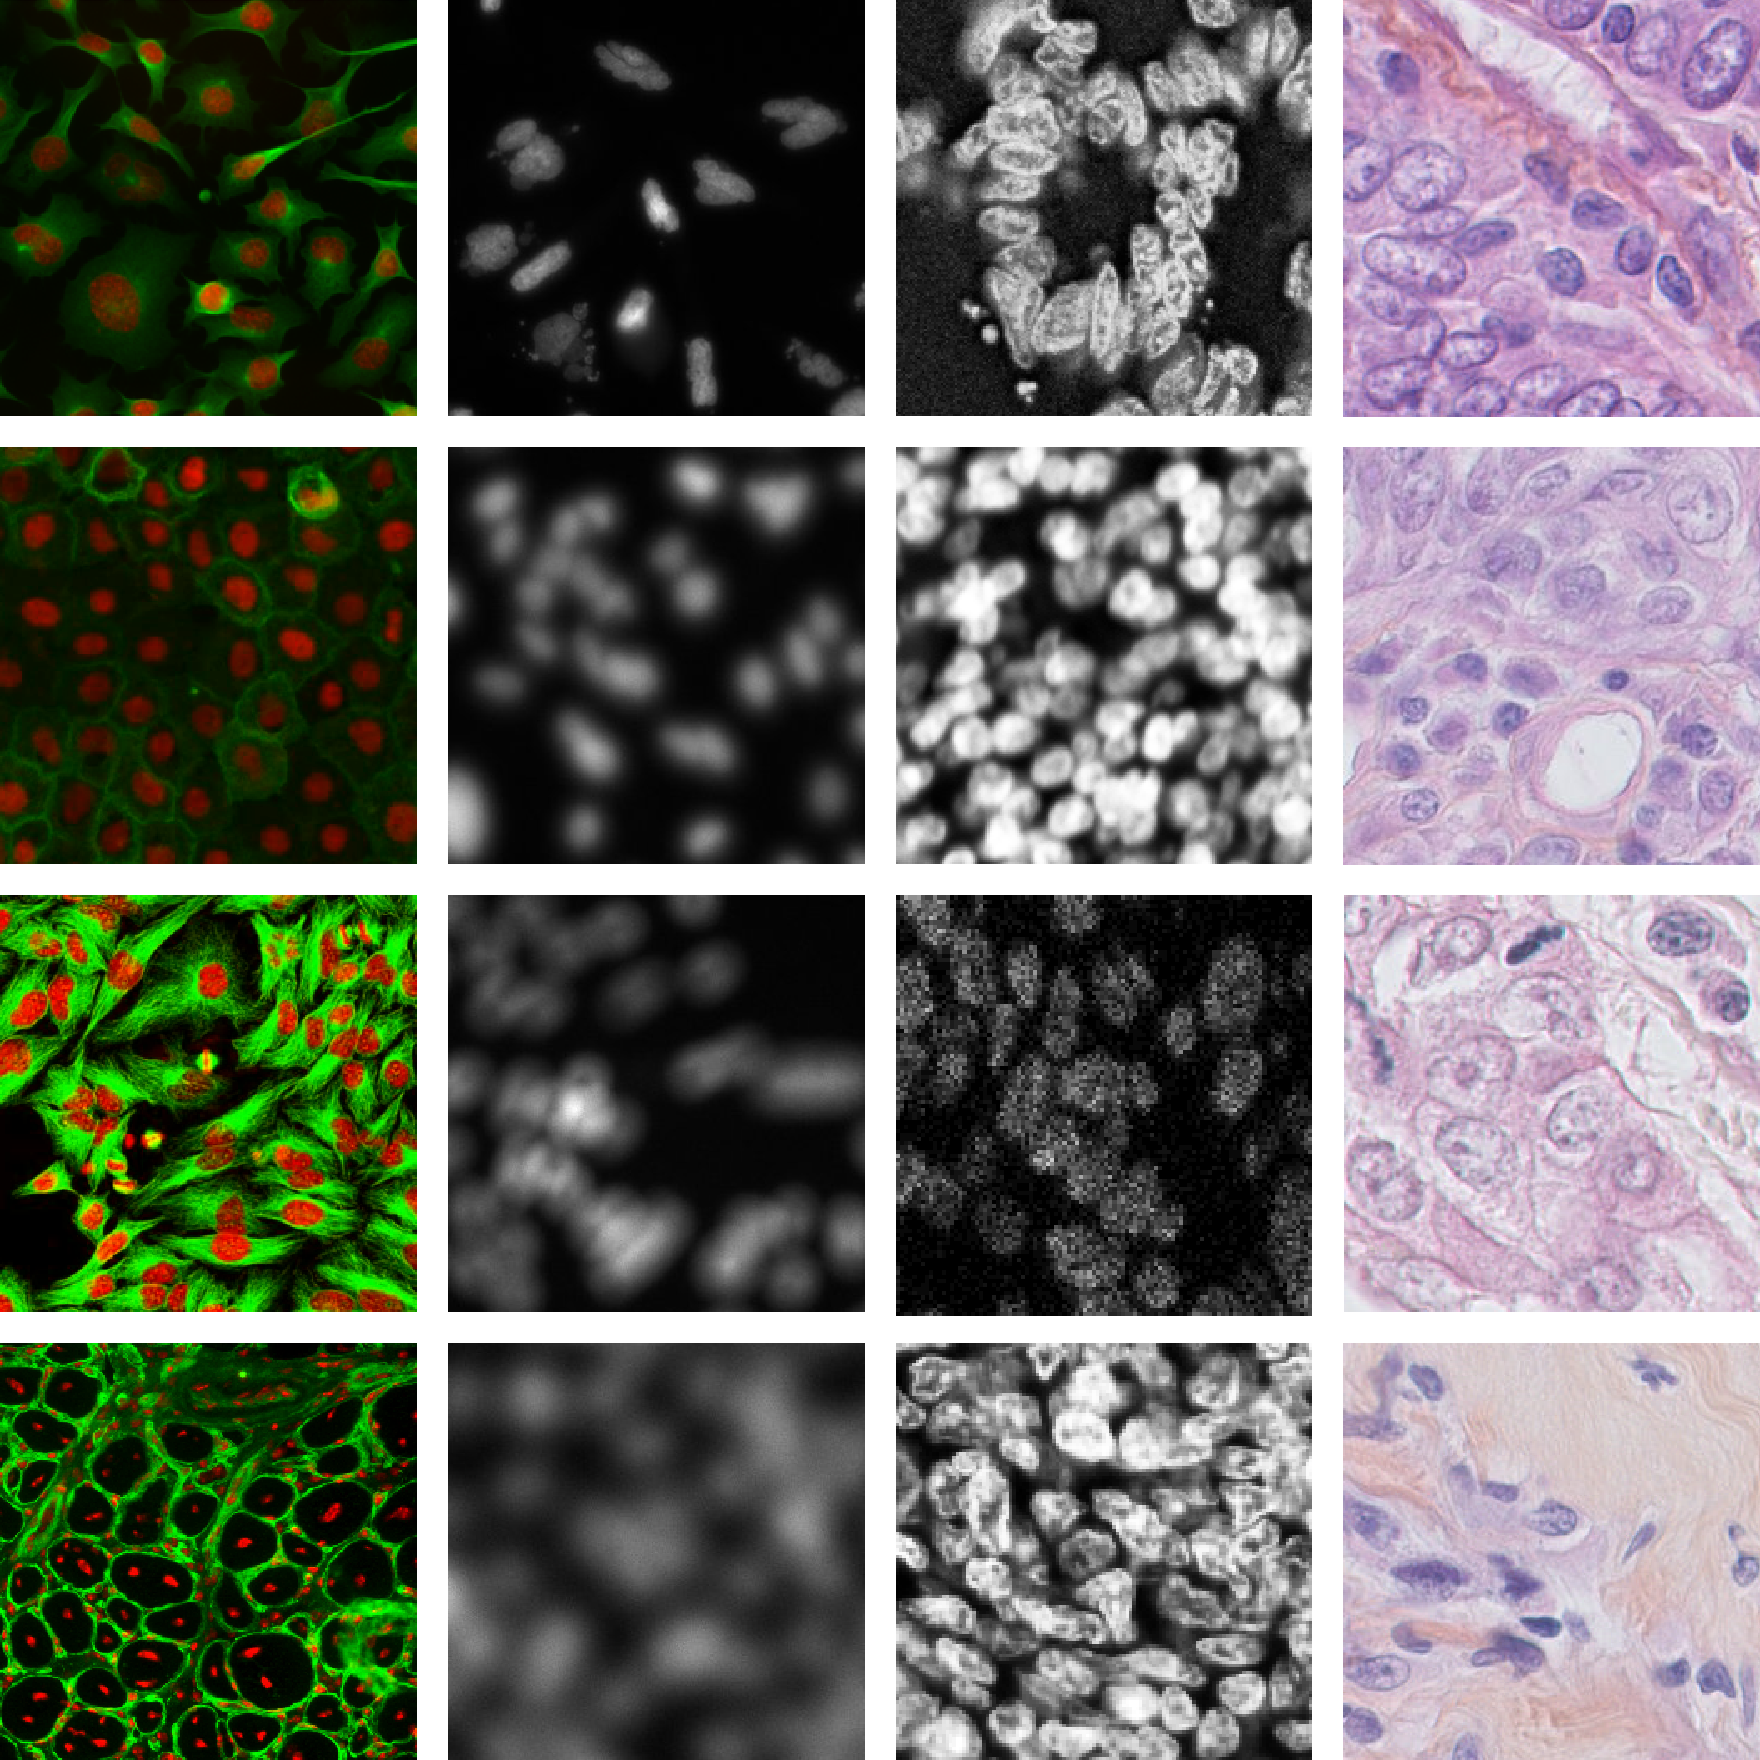
\includegraphics[width=\linewidth]{figs/Modality_Samples_4x4.pdf}
    \caption{\textbf{Illustating variability across microscopy imaging modalities and types.} First column describes images collected from Cellpose Gen. data~\cite{stringer2021cellpose}, second column represents various images of Human U20S cells with Hoechst and phalloidin stains from BBBC006~\cite{ljosa2012annotated}, the third column illustrates images from  Tissuenet~\cite{greenwald2022whole}, and the forth column shows results obtained using H \& stain from TNBC~\cite{naylor2018segmentation}.}
    \label{fig:modality}
\end{figure}


We are interested in improving tasks such as cellular activity monitoring. Various microscopes can be employed to produce videos of time-sequence observations in 2D and 3D volumes. For example, light-sheet, fluorescent, or confocal microscopy, each requiring tracking the cells in the volume they occupy. In \Cref{fig:modality}, we show different imaging data obtained using different platforms and on different tissue types. Given the variability among cells, which can differ in size and shape as well as in imaging modalities, it is evident that no single method can be generalized for all types of cell monitoring. According to \cite{bragantini2024ultrack}, this issue largely stems from the low-quality segmentation algorithms that introduce noise into the predictions, making it difficult to accurately link cells for lineage tracking. We align with this perspective and propose to address the test-time adaptation problem in cell instance segmentation to improve cell tracking in this manuscript.
 
\section{Methods}

\subsection{Overview}
Our hypothesis is that performing test time adaptation on cell segmentation will improve cell tracking performance since the associations are based on simple metrics such as IoU and Euclidean distance of the centroids~\cite{bragantini2024ultrack}. In our approach, we assume to have a pre-trained network available that was trained on a source dataset. Given that Cellpose~\cite{stringer2021cellpose} remains one of the leading algorithms for cell instance segmentation, we have selected it as our baseline algorithm and will build our TTA framework on top of it. In the sections that follow, we will provide an overview of the fundamentals of Cellpose~\cite{stringer2021cellpose}, discuss TTA, and outline our proposed framework.



\subsection{Cell Segmentation}

To test our hypothesis, we use one of the state-of-the-art cell instance segmentation algorithms as our segmentation framework Cellpose~\cite{stringer2021cellpose}. It is pretrained on diverse datasets and has good generalization capability. However, it is not pretrained on all imaging modalities or cell types, rendering it less useful in out-of-distribution datasets. We propose to utilize their pretrained model and perform test-time adaptation. 

Here, we describe the inner workings of Cellpose~\cite{stringer2021cellpose}: given an image $I$, the model uses a network $f$ to generate a dense, pixel-wise feature map $\bm{Z} = f(I)$, where $ \bm{Z} = [Z_1, Z_2, Z_3] \in \mathbb{R}^{h \times w \times 3}$. For some pixel $i$, we denote the feature $\mathbf{z} = [z_1, z_2, z_3] \in \bm{Z}$. Here, $\bm{z} \doteq (z_1, z_2)$ represents the gradient pointing towards the center of the cell structure to which pixel $i$ belongs. Together, $(Z_1,Z_2)$ form a \emph{gradient flow}. The component $z \doteq z_3$ represents the unnormalized score indicating the probability that pixel $i$ is part of a cell structure. It is worth noting that with this notation, the feature $\mathbf{z}$ can be written as $\mathbf{z} = [\bm{z}, z]$. The network $f$ is trained in a supervised manner with pixel-wise instance segmentation loss defined as follows:
\begin{equation}
 \mathcal{L}_i^{IS} = (z_1 - \mathtt{g_x})^2 + (z_2 - \mathtt{g_y})^2 + \nu H(\mathtt{m},\sigma(z))  \; ,
\end{equation}
where, for pixel $i$,  $(\mathtt{g_x}, \mathtt{g_y})$ represents the ground-truth gradient label with unit $\ell_2$-norm, $\mathtt{m} \in \{0, 1\}$ is the binary mask label indicating absence or presence of a cell structure, and $\sigma(z) \doteq 1/(1+\exp(-z))$ is the sigmoid function. The term $H$ represents the binary cross-entropy, and $\nu$ is a hyperparameter set to $0.04$. The contributions to the pixel-wise loss are aggregated into a final loss, $\mathcal{L}^{IS} = \sum \mathcal{L}_i^{IS}$ for the image $I$.


Given the feature $\bm{Z}$, the cell instance segmentation head $g$ produces the mask $Y = g(\bm{Z})$. For each pixel $i$, the predicted label $y$ takes the value from the set $\{0, 1, \cdots, N \}$, where $N$ represents the total number of segmented cell instances. Pixels that belong to the same cell instance share the same label, and $y=0$ indicates the absence of a cell instance. 


\subsection{Test-Time Adaptation Loss Computation}

At test-time, we follow two TTA constraints: \\
\indent (i) no source data available and \\
\indent (ii) no target labels available \\
In this setting, we want to perform the adaptation in a fully unsupervised manner. Once we have a pre-trained Cellpose~\cite{stringer2021cellpose} model available, we will utilize its predictions on the target data to perform the adaptation. 

\subsubsection{Self-Entropy}\label{sec:tta-se}
One of our first objectives is to calculate the Shannon entropy~\cite{shannon1948mathematical} of the mask probability predictions. Shannon entropy~\cite{shannon1948mathematical} allows us to quantify the model uncertainty in the model predictions. As it refers to the uncertainty of the model, we could also utilize this information as a metric to decide which predictions are confident predictions. It is especially crucial as data distributions can change during inference. As our mask predictions are given by $\sigma(z)$, our Shannon entropy~\cite{shannon1948mathematical} becomes the following:

\begin{equation}
    \mathcal{L}_i^{SE} = -\sigma(z) \log \sigma(z) \; ,
\end{equation}

However, since our mask predictions refer to a binary crossentropy task and do not possess a probability distribution over $k$ classes, we redefine the entropy as the following:
\begin{equation}
    \mathcal{L}_i^{SE} = -(\sigma(z) \log \sigma(z) + (1-\sigma(z)) \log (1-\sigma(z))) \; ,
\end{equation}

Now that we calculated $\mathcal{L}^{SE}$ for the binary mask predictions, we can use this information to collect more confident prediction. We choose a threshold $\delta$ that describes if the $\mathcal{L}_i^{SE}$ is lower than the threshold, then the predictions are confident enough. It is given by $\hat{\bm{z}} = \bm{z}[\mathcal{L}^{SE}<\delta]$. Further, once the indices are collected, we choose a probability threshold $p$ that determines if the original predictions have large enough probability to be considered a valid prediction which is given by $\hat{\bm{z}} = \hat{\bm{z}}[\sigma(z)>p]$. Now, we have a refined set of indices which will be useful in the next section. 

\subsubsection{Contrastive Flow Loss} \label{sec:tta-cfl}
The proposed framework utilizes a contrastive prediction task to enhance the gradient flow features of target pixels.  CellTranspose~\cite{keaton2023celltranspose} was the first to introduce a contrastive objective for the gradient flow alignment task, and we adopt their formulation in this paper. However, unlike their supervised framework, our approach employs contrastive learning in a self-supervised manner. \\

In our method, we define a positive sample using a refined binary mask from $\hat{z}$, represented as $\mathbb{I}[\hat{z}>p]$, which we denote as $\hat{z_+}$ (where $\hat{z} > p$). We then identify the gradient flow features $\hat{\bm{z}}_+$ that are closest to the prediction $\hat{\bm{z}} = (z_1, z_2)$ using a similarity metric. Specifically, we utilize cosine similarity, defined as $s(\bm{u}, \bm{v}) \doteq \frac{\bm{u}^T \bm{v}}{\| \bm{u} \| \| \bm{v} \|}$, with $\| \cdot \|$ denoting the $l_2$-norm. Next, we compile a set of negative samples $\mathcal{N}_i = \{\hat{\bm{z}}_- \; | \; s(\hat{\bm{z}}_+, \hat{\bm{z}}_-) < \theta, \hat{z}_- > p\}$, where $\theta$ is a hyperparameter threshold that we select. After gathering the positive and negative samples, we apply our contrastive objective for pixel $i$, aiming to pull the positive pairs $(\hat{\bm{z}}, \hat{\bm{z}_+})$ closer together while pushing the negative pairs $(\hat{\bm{z}}, \hat{\bm{z}}_-)$ apart. \\

Furthermore, \cite{wang2021understanding} recommends effective hard-mining strategies for learning with a contrastive objective. By implementing hard-mining for negative samples, we can reduce the need for a large number of negative samples while enhancing convergence speed. Since our objective adapts at test time, rapid convergence greatly benefits the algorithm. Therefore, similar to \cite{keaton2023celltranspose}, we adopt a hard-mining sampling strategy for negative samples. Essentially, $\mathcal{N}_i$ consists of pixels that are in close proximity to the positive samples. For more details, please refer to \cite{keaton2023celltranspose}.\\

Given a batch of target image patches, each patch is paired with another patch from the same batch. We then compute the contrastive flow loss aggregating all the components coming from all the valid pixels, i.e.,  $\hat{z}_- > p$. 
Now the loss function becomes the following:

\begin{equation}
    \small
    \mathcal{L}_i^{CF} = - \log \frac{\exp( s (\hat{\bm{ z}}, \hat{\bm{ z}}_+)/\tau )}{ \exp( s (\hat{\bm{ z}}, \hat{\bm{ z}}_+)/\tau ) + \sum_{\hat{\bm{ z}}_- \in \mathcal{N}_i} \exp( s (\hat{\bm{ z}}, \hat{\bm{ z}}_-)/\tau ) }\\
    \label{eq-contrastive-flow-loss}
  \end{equation}
where $\tau$ refers to a temperature parameter we choose. 

\subsubsection{Adaptation Loss}
In \cref{sec:tta-se}, we calculate self-entropy for the binary mask predictions and in \Cref{sec:tta-cfl}, we calculate a contrastive object to enhance the gradient flow estimations. We combine this two losses for the model update at test time as shown below:
\begin{equation}
    \small
    \mathcal{L}^{TTA} = \lambda_1\frac{1}{| \mathcal{M}_1 |} \sum_{\mathcal{M}_{1}} \mathcal{L}^{SE}_i + \lambda_2\frac{1}{| \mathcal{M}_2 |} \sum_{\mathcal{M}_2} \mathcal{L}^{CF}_i \; .
    \label{eq-tta-loss}
  \end{equation}
Where, total pixel belonging to the target patch, we define it by $\mathcal{M}_1$, and the valid pixels we define that set by $\mathcal{M}_2$. $\lambda_1$ and $\lambda_2$ are the weight parameters for the loss. This combination of losses is used to perform the adaptation. In the next section, we will discuss what parameters we want to update during TTA. 

\subsection{Test-Time Adaptation Parameter Updates}
Studies have shown that the major cause of performance degradation in convolution-based networks is the shift in batch-normalization statistics during inference~\cite{wang2020tent,niu2022efficient,zaveri2025improving,li2016revisiting,mirza2022norm,pan2018two,schneider2020improving}. We take advantage of these findings and propose to only update the batch-normalization parameters. They are calculated by the following equations:

\begin{equation}\small
    \centering
    \label{eq:bn}
        \begin{aligned}  
        BN(x) = \gamma \frac{x - E(x)}{\sqrt{Var(x)}} +  \beta ,
        \end{aligned}
\end{equation}
\begin{equation}\small
    \centering
    \label{eq:bn_running}
        \begin{aligned}  
            \overline{\mu}_t = (1-\alpha)  \overline{\mu}_{t-1} +  \alpha  {\mu}_t ,\\
            \overline{\sigma}_{t}^2 = (1-\alpha) \overline{\sigma}_{t-1}^2 +  \alpha {\sigma}_{t}^2 ,
        \end{aligned}
\end{equation}

where $x$ is the input feature, $E(x)$ and $Var(x)$ are the expected value and variance of $x$. $\gamma$ and $\beta$ are learnable parameters for scaling and shifting. The BN layers keep track of the running mean and variance through Equation \ref{eq:bn_running}, where ${\mu}_t$ and ${\sigma}_{t}$ are current expected value and variance respectively, and $\overline{\mu}_t$ and $\overline{\sigma}_{t}$ are used for $E(x)$ and $Var(x)$, respectively. $\alpha$ is the momentum parameter. We propose to estimate the learnable parameters $\gamma$ and $\beta$ during testing that requires a backward pass. Additionally, we also dynamically updates the BN statistics $E(x)$ and $Var(x)$ during testing according to the following strategy:
\begin{equation}
  \centering
  \label{eq:bn_update}
      \begin{aligned}  
          \overline{\mu}_{I,t} &= (1-\lambda{_{BN}}) \overline{\mu} +  \lambda{_{BN}} \mu_{I,t} \; ,\\
          \overline{\sigma}_{I,t}^2 &= (1-\lambda{_{BN}}) \overline{\sigma}^2 +  \lambda{_{BN}} \sigma_{I,t}^2 \; ,
      \end{aligned}
\end{equation}
where $\overline{\mu}$ and $\overline{\sigma}^2$ are the final running mean and variance of the model trained on the source data, respectively, and $\mu_{I,t}$, and $\sigma_{I,t}^2$ are mean and variance calculated from the instance at time $t$, respectively. $\overline{\mu}_{I,t}$ and $\overline{\sigma}_{I,t}^2$ are updated based on the current instance and used for feature normalization at time $t$. $ \lambda{_{BN}}$ is set to 0.1. 

\section{Experiments}
\subsection{Implementation}

We follow Cellpose~\cite{stringer2021cellpose} and utilize their U-Net architecture and the data to pretrain the network on a Titan Xp GPU for 500 iterations with a batch size of 8. Since our approach is considered a test-time adaptation approach, we adapt to test instances from the test split of various benchmarks we evaluate in this manuscript. We use SGD with the learning rate of 0.01, momentum 0.9, weight decay of 0.00001, and batch size of 2. We take square patches of size $h=w=112$, with a minimum overal of 48 during evaluation, and nominal cell size $m_n = 30$. Hyperparameters for adaptation losses are $\lambda_1 = \lambda_2 = 1.0$.  Following ~\cite{keaton2023celltranspose}, we set other hyperparameters as: $|\mathcal{N}_i|=20, \tau=0.1$, and $\theta=0.05$.

\subsection{Evaluation Metrics}
Following Cellpose~\cite{stringer2021cellpose}, we quantify our predictions by matching our predicted masks with the ground truth masks, and whichever provides the highest IoU becomes the pair we consider as true positive (TP). The masks without any valid matches are false positives (FP), and the ground truth masks without any valid matches are considered false negatives (FN). With these predictions defined, we compute the standard average precision metric AP for each image and then average it as defined below:
\begin{equation}
    AP = \frac{TP}{TP+FP+FN}
\end{equation}   
We also compute the F1 score which is given by:
\begin{equation}
    F1 = \frac{TP}{TP+\frac{1}{2}(FP+FN)}
\end{equation} 
\subsection{Datasets}
We choose Cellpose~\cite{stringer2021cellpose} Generalist dataset as our source data and \textbf{TissueNet}~\cite{TissueNet} data splits as our various domains we want to adapt to. TissueNet~\cite{TissueNet} collects tissue data (i.e., Breast, GI, Immune, Pancreas, etc.) from many platforms (i.e., CyCIF, CODEX, Vectra, MIBI, etc. ). We adapt to each of these specific domains separately in our experiments. In \Cref{tab:tn1,tab:tn2}, we show relative improvement over various dataset splits within TissueNet. The left portion describes the platform type and the right describes the tissue type. In each case, we show that we improve over the baseline. For example, for Codex-Pancreas, we improved from 0.717 to 0.742 in just one backward pass without any target labels or source data. We also present qualitative evaluation of our approach in \Cref{fig:qual}. In each of the cases illustrated, we can observe relatively low number of false positives and false negatives in the adapted version compared to the baseline. We also compare against CellTranspose~\cite{keaton2023celltranspose} which is a supervised few-shot adaptation approach for cell instance segmentations. We use 3-shot setting and showcase their performance in  \Cref{tab:tn1,tab:tn2}. We can notice that CellTranspose is significantly better than Cellpose and Cellpose-tta; however, it was expected as our TTA setting is fully unsupervised and CellTranspose is supervised. However, it does lead us to a question in terms of is accuracy trade-off useful is it only takes a few minutes to annotate the data. We will leave the discussion as future works. 

\begin{table}
    
    \caption{Comparative analysis on various splits of TissueNet. We show improvement with test-time adaptation. }
    \label{tab:tn1}
    \scalebox{0.8}{
\begin{tabular}{c|cc|cc|cc}
    CP $\rightarrow$ TN  & \multicolumn{2}{l|}{Codex-Pancreas} & \multicolumn{2}{l|}{CyCIF-Immune} & \multicolumn{2}{l}{MIBI-Breast} \\
                            & {AP}             & F1                    & {AP}             & F1                    & {AP}             & F1                    \\ 
\hline
Cellpose                  & {0.717}          & 0.836                 & {0.476}          & 0.640                 & {0.228}          & 0.346                 \\
Cellpose-tta              & {\textbf{0.742}} & \textbf{0.853}        &{\textbf{0.501}} & \textbf{0.661}        & {\textbf{0.239}} & \textbf{0.361}        \\ 
\hline
CellTranspose             & 0.852              &  0.926 &        0.816       & 0.899 & 0.662 & 0.799 \\
\end{tabular}
    }
\end{table}

\begin{table}
    
    \caption{Comparative analysis on various splits of TissueNet. We show improvement with test-time adaptation. }
    \label{tab:tn2}
    \scalebox{0.8}{
\begin{tabular}{c|cc|cc|cc}
    CP $\rightarrow$ TN  & \multicolumn{2}{l|}{Mixif-GI} & \multicolumn{2}{l|}{Vectra-Immune} & \multicolumn{2}{l}{Vectra-Breast} \\
                            & {AP}             & F1                    & {AP}             & F1                    & {AP}             & F1                    \\ 
\hline
Cellpose                  & {0.355}          & 0.527                 & {0.629}          & 0.776                 & {0.574}          & 0.745                 \\ 
Cellpose-tta              & {\textbf{0.373}} & \textbf{0.545}        &{\textbf{0.631}} & \textbf{0.777}        & {\textbf{0.583}} & \textbf{0.751}        \\ 
\hline
CellTranspose             &    0.697            & 0.827 &    0.858          & 0.924 & 0.821 & 0.909 \\
\end{tabular}
    }
\end{table}


\begin{figure}
    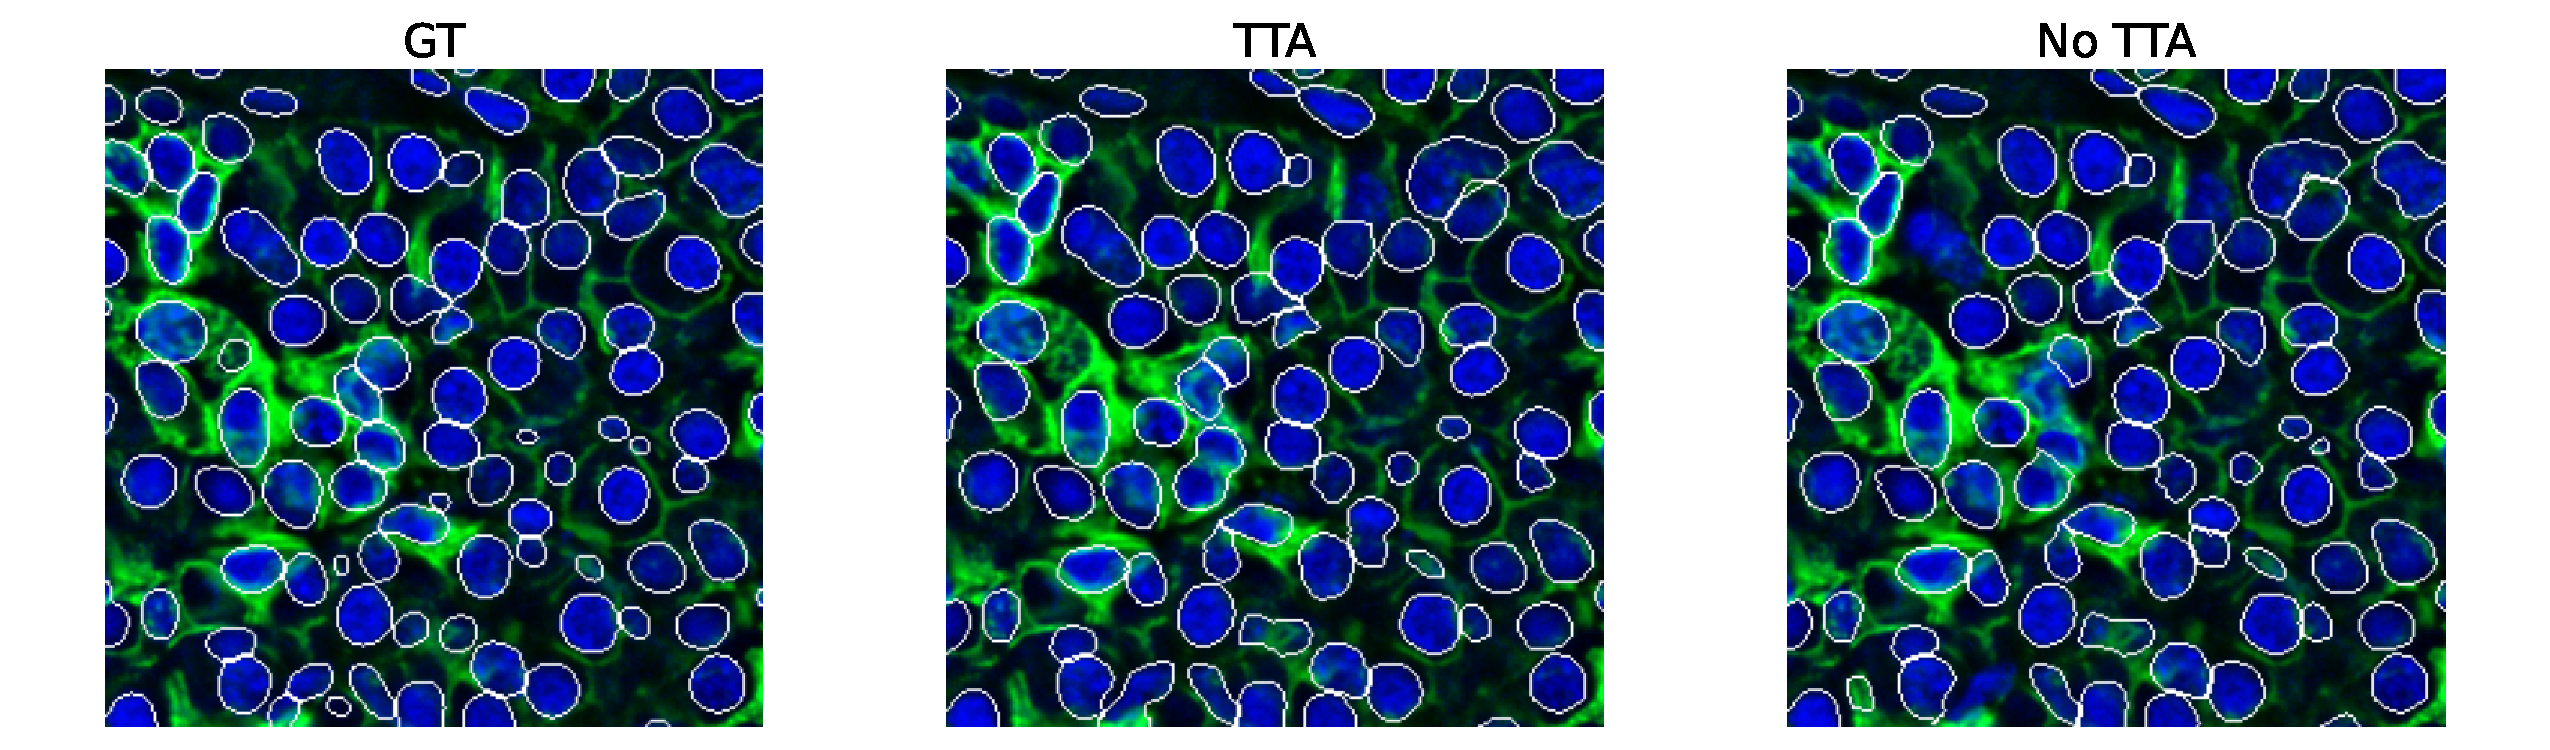
\includegraphics[width=8.75cm]{figs/1.pdf}
    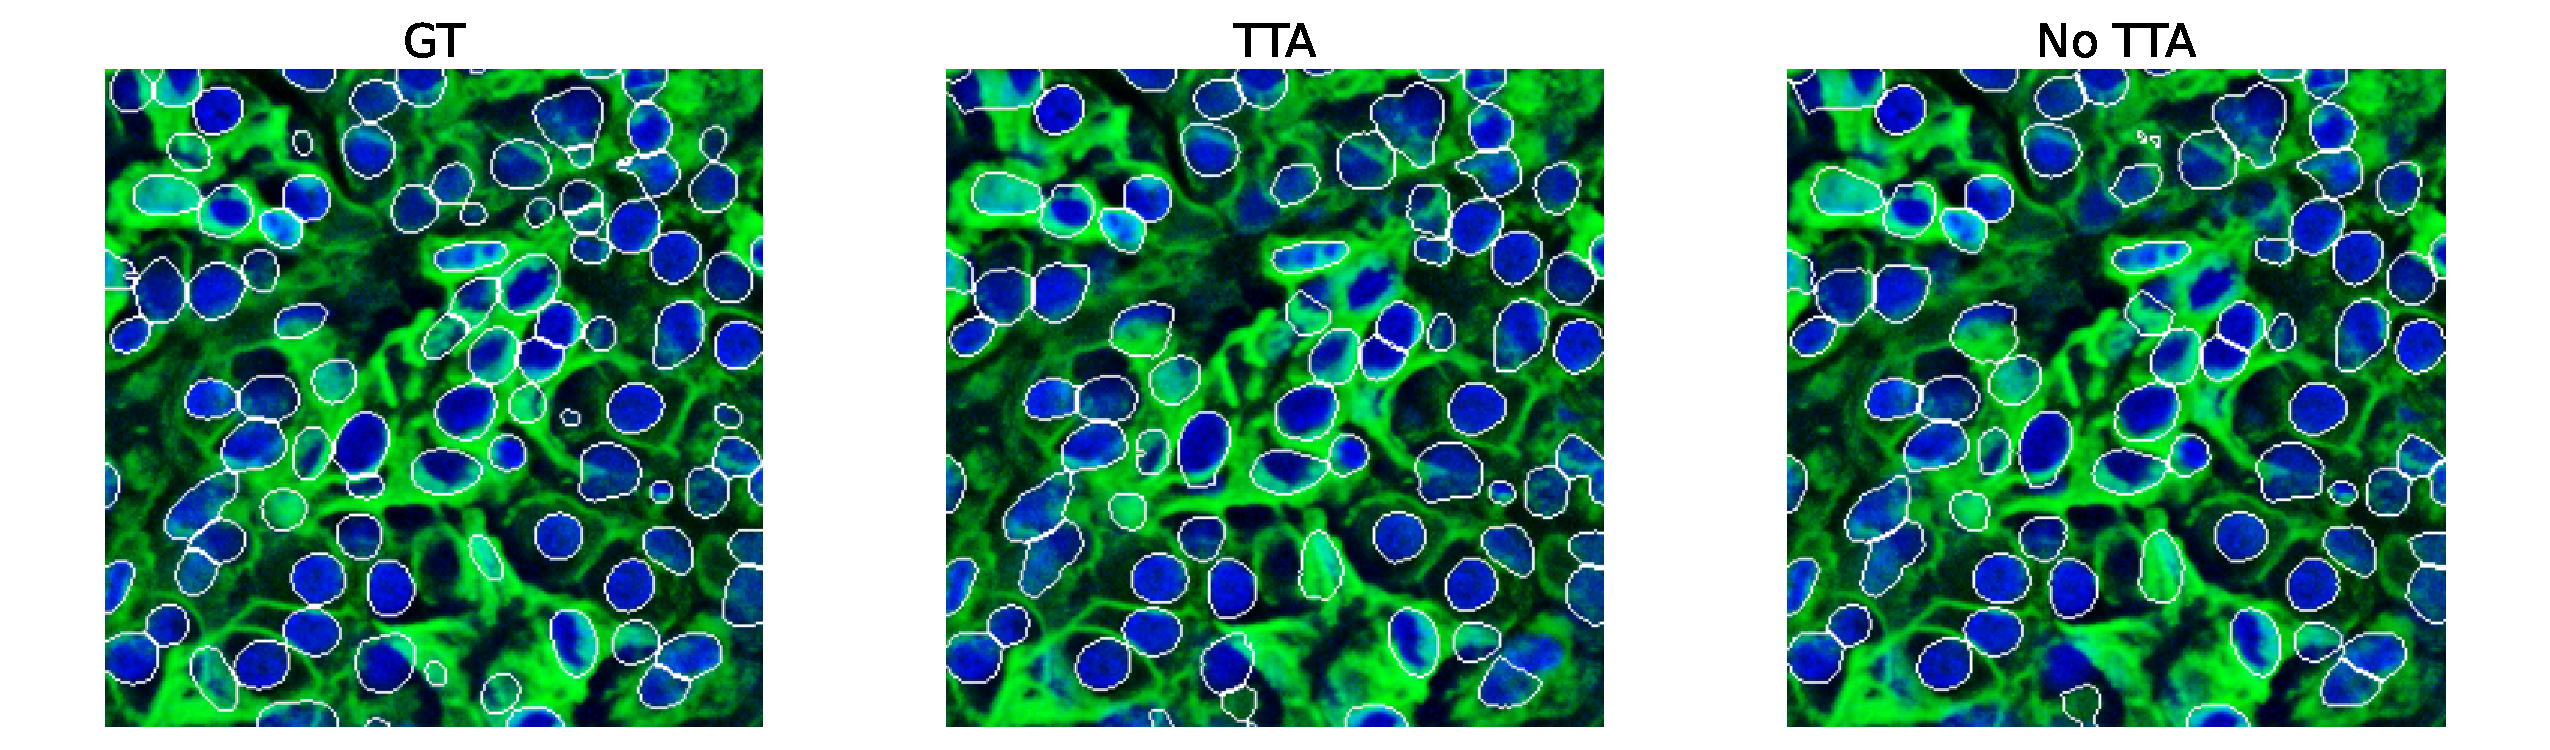
\includegraphics[width=8.75cm]{figs/43.pdf}
    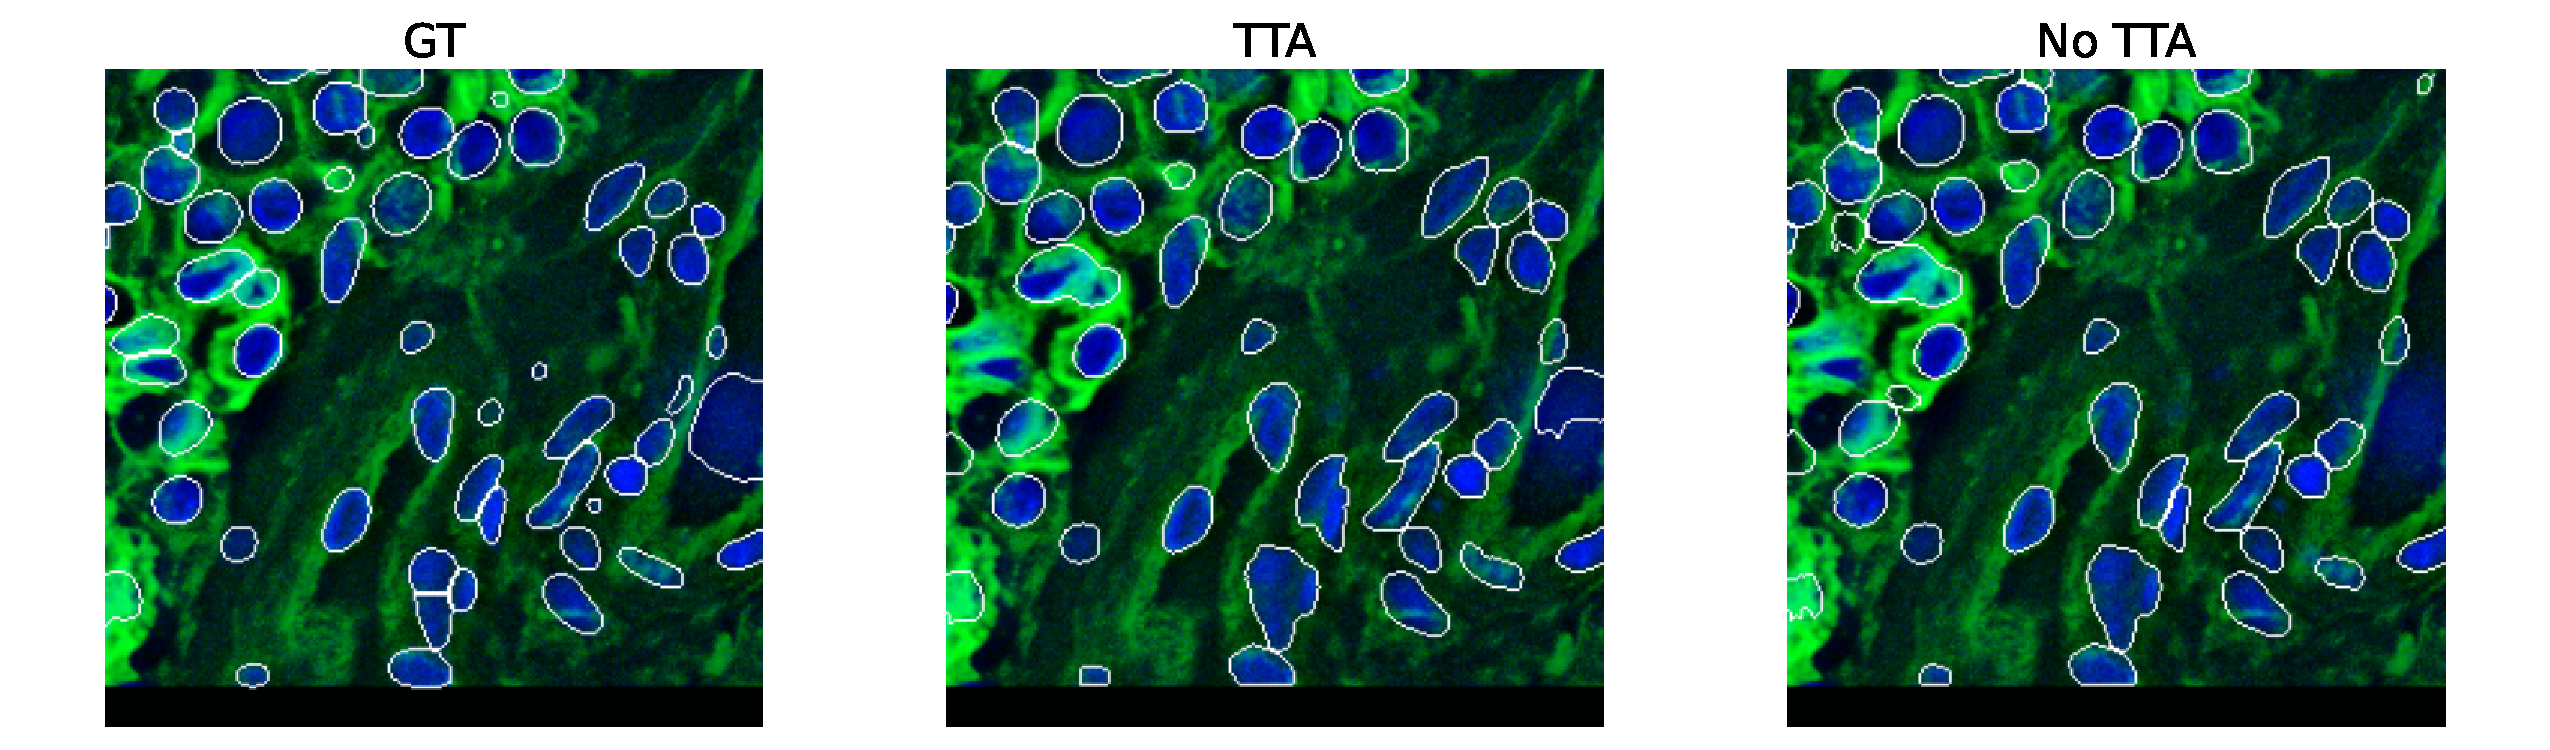
\includegraphics[width=8.75cm]{figs/45.pdf}
    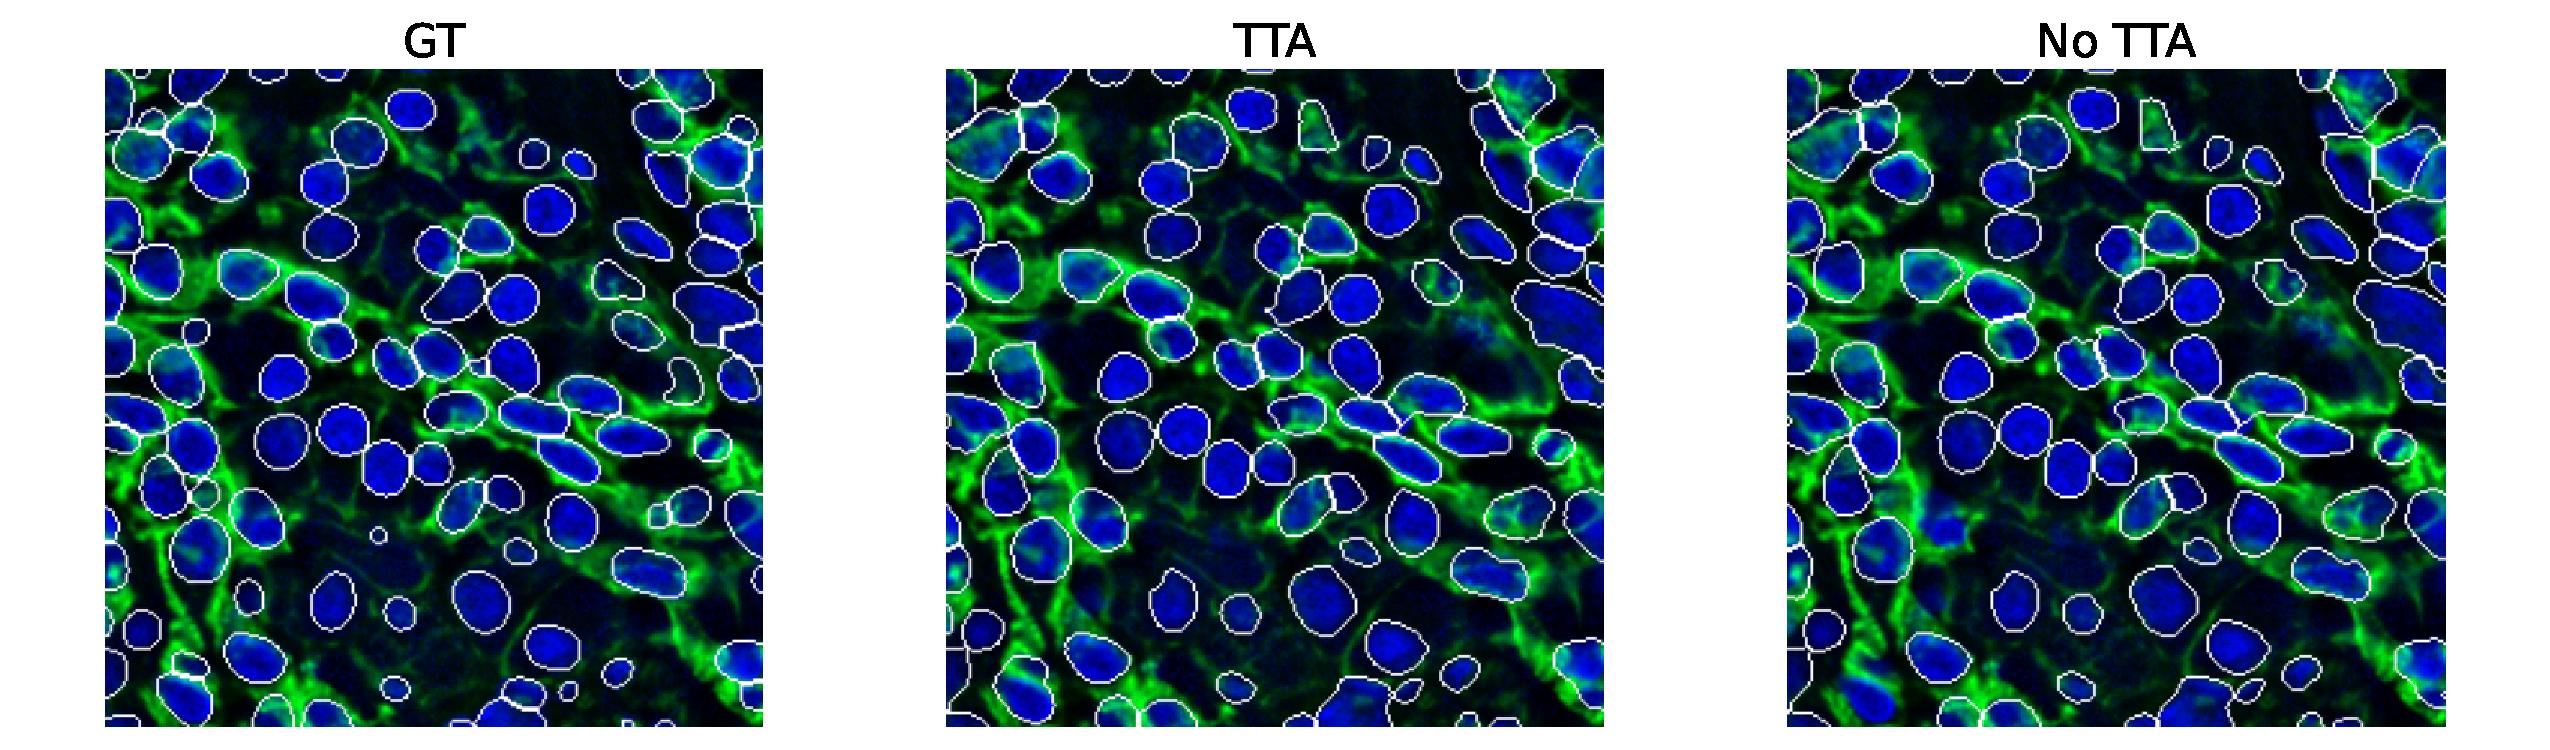
\includegraphics[width=8.75cm]{figs/55.pdf}
    \caption{\textbf{Illustating TTA results on Codex-Pancreas dataset from TissueNet against the ground truth and the baseline.} In each of the cases illustrated, we can observe relatively low number of false positives and false negatives in the adapted version compared to the baseline.}
    \label{fig:qual}
\end{figure}

\section{Conclusions}
\dots

{
    \small
    \bibliographystyle{ieeenat_fullname}
    \bibliography{main}
}

% WARNING: do not forget to delete the supplementary pages from your submission 
% \clearpage
\setcounter{page}{1}
\maketitlesupplementary


\section{Rationale}
\label{sec:rationale}
% 
Having the supplementary compiled together with the main paper means that:
% 
\begin{itemize}
\item The supplementary can back-reference sections of the main paper, for example, we can refer to \cref{sec:intro};
\item The main paper can forward reference sub-sections within the supplementary explicitly (e.g. referring to a particular experiment); 
\item When submitted to arXiv, the supplementary will already included at the end of the paper.
\end{itemize}
% 
To split the supplementary pages from the main paper, you can use \href{https://support.apple.com/en-ca/guide/preview/prvw11793/mac#:~:text=Delete%20a%20page%20from%20a,or%20choose%20Edit%20%3E%20Delete).}{Preview (on macOS)}, \href{https://www.adobe.com/acrobat/how-to/delete-pages-from-pdf.html#:~:text=Choose%20%E2%80%9CTools%E2%80%9D%20%3E%20%E2%80%9COrganize,or%20pages%20from%20the%20file.}{Adobe Acrobat} (on all OSs), as well as \href{https://superuser.com/questions/517986/is-it-possible-to-delete-some-pages-of-a-pdf-document}{command line tools}.

\end{document}
